%\noindent {\bf Requirements/Assumptions}: 
\subsection{Requirements/Assumptions}
This installation recipe assumes the availability of a single head node {\em
 master}, and four {\em compute} nodes. The {\em master} node serves as the
overall system management server (SMS) and is provisioned with \baseOS{} and is
subsequently configured to provision the remaining {\em compute} nodes with
\Warewulf{} in a stateless configuration. The terms {\em master} and SMS are
used interchangeably in this guide. For power management, we assume that
the compute node baseboard management controllers (BMCs) are available via IPMI
from the chosen master host. For file systems, we assume that the chosen master
server will host an \NFS{} file system that is made available to the compute
nodes. Installation information is also discussed to optionally include a
\Lustre{} file system mount and in this case, the \Lustre{} file system is
assumed to exist previously.

\begin{figure}[hbt]
\center
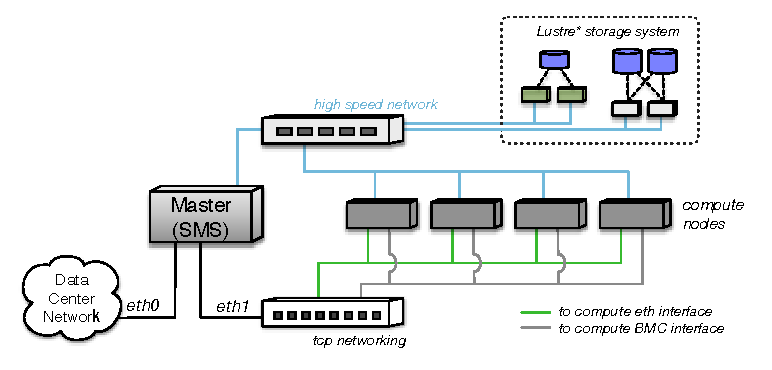
\includegraphics[width=0.8\linewidth]{ohpc-arch-small2.pdf}
\vspace*{-0.2cm}
\caption{Overview of physical cluster architecture.} \label{fig:physical_arch}
\end{figure}
\mbox{}

An outline of the physical architecture discussed is shown in
Figure~\ref{fig:physical_arch} and highlights the high-level networking
configuration. The {\em master} host requires at least two Ethernet interfaces
with {\em eth0} connected to the local data center network and {\em eth1} used
to provision and manage the cluster backend (note that these interface names
are examples and may be different depending on local settings and OS
conventions). Two logical IP interfaces are expected to each compute node: the
first is the standard Ethernet interface that will be used for provisioning and
resource management. The second is used to connect to each host's BMC and is
used for power management and remote console access. Physical connectivity for
these two logical IP networks is often accommodated via separate cabling and
switching infrastructure; however, an alternate configuration can also be
accommodated via the use of a shared NIC, which runs a packet filter to divert
management packets between the host and BMC.

 In addition to the IP networking, there is a high-speed network
(\InfiniBand{} in this recipe) that is also connected to each of the
hosts. This high speed network is used for application message passing and
optionally for \Lustre{} connectivity as well.

